%The charge within each pixel on a sensor is collected through the estimation of the photons impinging on the respective pixel surface, inversely proportional to the capacitance ....
%A photon with energy hν breaks a silicon bond and frees both an electron (e-) and a hole (e+).
Imaging electronic devices consist of arrays of pixels, consisting of photodiodes accumulating charge through incoming light and integrated circuits which read out the charge and process it further.

For the accumulation of charge, the properties of the semiconductor materials are exploited. 
The unique electrical conductivity of semiconductors can be altered significantly through external sources of energy, e.g. thermally or by light illumination, and increases proportionally. 

The incident photons impinge on the surface of the image sensor and are absorbed through the corresponding structures in the semiconductor material, creating electron-hole pairs as the electron is excited from the valence to the conduction-band. The photoexcited carriers remain within the sample; this is called \textit{internal photoeffect}. \cite{Saleh1991} %645 & 576 %to the higher energy level.

Electrical and optical properties of the semiconductors can be altered further through \textit{doping}, an adding of local impurities for changed concentration of the carriers. In semiconductors, selective doping creates an electrostatic potential well. Subjected to the externally applied electric field, the freed photoelectrons drift through the material towards the potential well, where they are stored and integrated for the duration of exposure. This photoelectron charge is later transferred to the sense capacitance, thus producing measurable electric current through changes in the charge on the charge sense node (\textit{floating diffusion} FD) and converting the signal to voltage, which is read out by the a source follower transistor. \cite{9059308} %their charge is converted to voltage via transfer to a sense capacitance, change in the charge on this sense node causes change in voltage, thus converting the signal from charge domain to voltage domain

The outputs of the source-followers are amplified and fed to the signal processing circuits on a greater scale, allowing the separate pixels to be adressed column-wise. After the integration, the pixels are reset.

\begin{figure}[h]
  \centering
  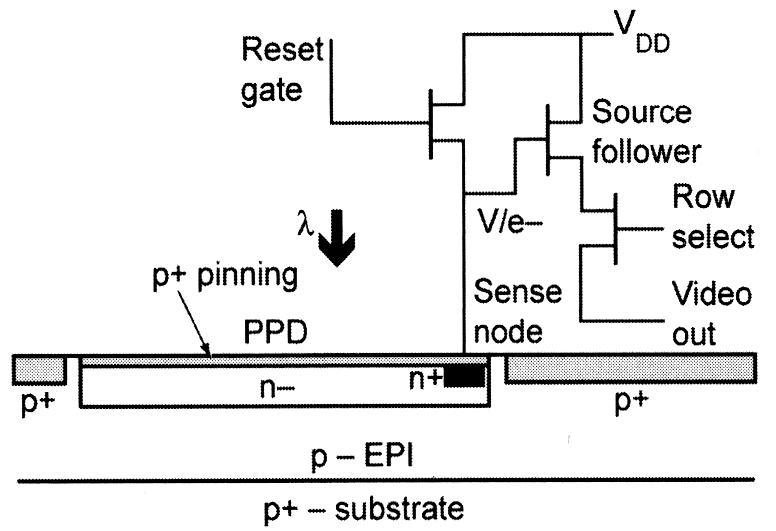
\includegraphics[width=0.9\linewidth]{imgs/sensors/3tppd.png}
  \caption{3T PPD structure, via \cite{Holst2011}. Typically, the dark current is heightened through the direct n+ contact; here, this is prevented through p+-pinning structure on the pixel surface.}
  \label{fig:3tppd}
  \Description{The classical pinned photodiode structure with three nodes.}
\end{figure}

Many implementations for the photodiodes exist. In the simplest pixel circuit, three transistors (3T: source-follower, reset, and row select transistors) are needed for the integration process. Modern CIS technologies make use of 4T pinned photodiode structure, in which an additional transfer gate is positioned between photodiode and the sense node. This ensures reduction of dark current and complete charge transfer; the ``pinning'' of the photodiode allows for reduced sense node capacitance. 
Furthermore, with this design structure, the pixels can be reset simultaneously, allowing for same integration periods globally.

\begin{figure}[h]
  \centering
  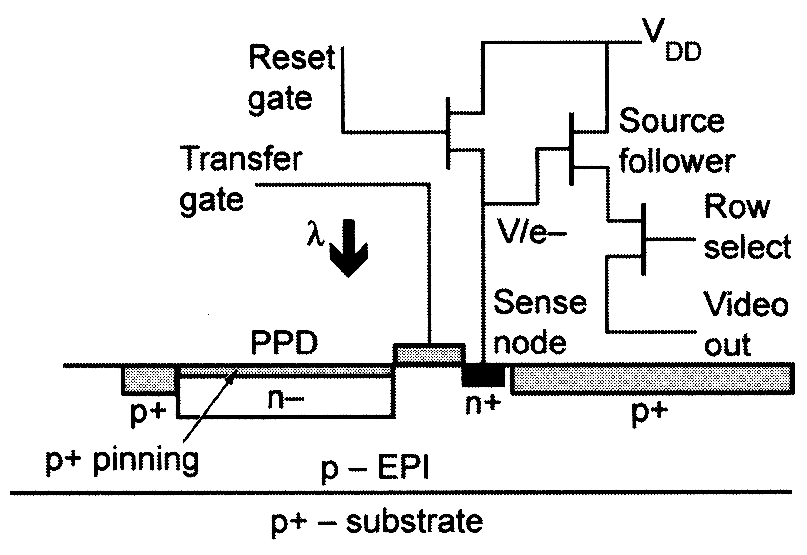
\includegraphics[width=0.9\linewidth]{imgs/sensors/4tppd.png}
  \caption{4T PPD structure, via \cite{Holst2011}. The transfer gate provides isolation of the regions.}
  \label{fig:4tccd}
  \Description{The pinned photodiode structure with four transistors. There are slight differences regarding the placement of the wells and the junctions, as the n+ is now spatially separated from the n-.}
\end{figure}

Only a fraction of the incident photon flux is absorbed and brought to a higher energy level. The ratio of the photoelectrons to the incident photons is given by \textit{quantum efficiency} (QE), which often ranges from 50\% to 80\% \cite{9059308}.
The relationship between the changes in output voltage caused by the photoelectric effect to the number of photoelectrons is given by conversion gain (CG); in modern CIS devices, this typically amounts to 100$\mu$V/$e^{-}$~\cite{7006672}. 
